\appendix
%███████████████████████████████████████████████████████████████████
%███████████████████████████████████████████████████████████████████
%███████████████████████████████████████████████████████████████████
\chapter{Overview of Aberration equations}

\section{Aberration Equations}
\section{Vectors}
\begin{equation}%%%%%%%%%%%%%%% 
\label{retarded displacement 2}
    \Vec{R}'_{ret}= \begin{pmatrix}
    x\\ y \\ \gamma \left(z + \dfrac{u_p \cdot \|\vec{R}\|}{c}\right)
    \end{pmatrix} = \|\vec{R}\|\begin{pmatrix}
    \frac{x}{\|\vec{R}\|}\\ \frac{y}{\|\vec{R}\|} \\ \gamma \left( \frac{z}{\|\vec{R}\|} + \dfrac{u_p}{c} \right)\\
    \end{pmatrix}.
\end{equation}%%%%

\begin{equation}%%%%%%%%%%%%%%% 
\label{eq: unit retarded velocity 2}
    \hat{\mathbf{\vec{U}'}} = \hat{\mathbf{\vec{R}'}}_{ret} = \dfrac{1}{\text{\AA}} \begin{pmatrix}
    \frac{x}{\|\vec{R}\|}\\ \frac{y}{\|\vec{R}\|} \\ \gamma \left( \frac{z}{\|\vec{R}\|} + \dfrac{u_p}{c} \right)
    \end{pmatrix},
\end{equation}%%%%

\begin{equation}%%%%%%%%%%%%%%%
\label{eq: field displacement transform 2}
    \|\Vec{R}'_{ret}\|^2 = \text{\AA}^2 \|\vec{R}\|^2
\end{equation}%%%%

\section{Trig}
\begin{equation}%%%%%%%%%%%%%%%
    \text{\AA} = \gamma\left(1+\dfrac{u_p}{c}\cos\theta\right) = \gamma\left(1-\beta\cos\theta\right) = \frac{1}{\gamma\left(1+\beta\cos\theta^{'}\right)}
\end{equation}%%%%


\begin{equation}%%%%%%%%%%%%%%%
\label{A Cosine transform}
    \cos\theta' = \dfrac{\cos\theta + \dfrac{u_p}{c}}{1+\dfrac{u_p}{c}\cos\theta} = \dfrac{\cos\theta - \beta}{1-\beta\cos\theta}
\end{equation}%%%%

\begin{equation}%%%%%%%%%%%%%%%
\label{Reverse Cosine transform}
    \cos\theta = \dfrac{\cos\theta' - \dfrac{u_p}{c}}{1-\dfrac{u_p}{c}\cos\theta'} = \dfrac{\cos\theta' + \beta}{1+\beta\cos\theta'}
\end{equation}%%%%

\begin{equation}%%%%%%%%%%%%%%%
\label{Sine transform}
    \sin\theta = \dfrac{\sin\theta'}{\gamma \left(1+\beta\cos\theta'\right)} = \text{\AA}\sin\theta'
\end{equation}%%%%

\section{Differential}


\begin{equation}%%%%%%%%%%%%%%%
\label{Differential transform}
    d\theta' = \dfrac{1}{\text{\AA}} d\theta
\end{equation}%%%%

%███████████████████████████████████████████████████████████████████
%███████████████████████████████████████████████████████████████████
%███████████████████████████████████████████████████████████████████
\chapter{Generalised Lorentz Vector Transformations}

\section{Lorentz boost}
The general transformation of the coordinates from the initial( (proper?) frame, $\vec{X}_0 = (ct_0,x_0,y_0,z_0)$, to coordinates, $\vec{X}_{\langle ' \rangle} $ in frame moving at $\vec{v}=(v_x,v_y,v_z)$ is given by; $\vec{X}_{\langle ' \rangle} = \vec{B}(\vec{v})\vec{X}_0$, where $\vec{B}(\vec{v})$ is:
\begin{equation}%%%%%%%%%%%%%%%
    \vec{B}(\vec{v}) = \begin{pmatrix}
    \gamma & -\dfrac{\gamma v_x}{c^2}& -\dfrac{\gamma v_y}{c^2}&- \dfrac{\gamma v_z}{c^2} \\ 
    -\dfrac{\gamma v_x}{c^2} & 1+(\gamma-1)v^{2}_{x} & (\gamma-1)v_yv_x& (\gamma-1)v_xv_z \\
    -\dfrac{\gamma v_y}{c^2} & (\gamma-1)v_xv_y & 1+ (\gamma-1)v^{2}_{y}& (\gamma-1)v_yv_z \\
    -\dfrac{\gamma v_z}{c^2} & (\gamma-1)v_xv_z & (\gamma-1)v_yv_z & 1+(\gamma-1)v^{2}_{z}
    \end{pmatrix}
\end{equation}%%%%
Lorentz boost must only be used to transform from proper frame to primed frame??????? what is the inverse in this case?


\section{Coordinate Transform}

Starting with position vector $\vec{r} = (x,y,z)$ and $\vec{r} = \vec{r}_{\perp} + \vec{r}_{\parallel}$, where $\vec{r}_{\perp}$ is component perpendicular to velocity of primed frame, $\vec{v}= (v_x,v_y,v_z)$, in which you wish to transform into, and $\vec{r}_{\parallel}$ is the component that is parallel to this velocity. We then have from the one dimensional Lorentz transformation:
\begin{equation}%%%%%%%%%%%%%%%
    \vec{r}_{\parallel \langle ' \rangle}  = \gamma (\vec{r}_{\parallel}-\vec{v}t)
\end{equation}%%%%
and
\begin{equation}%%%%%%%%%%%%%%%
    \vec{r}_{\perp \langle ' \rangle}  = \vec{r}_{\perp}
\end{equation}%%%%
where 
\begin{equation}%%%%%%%%%%%%%%%
    \vec{r}_{\parallel}= \left( \vec{\hat{v}}\cdot\vec{r}\right)\vec{\hat{v}} =  \bigg(\dfrac{\vec{v}\cdot\vec{r}}{|\vec{v}|}\bigg)\dfrac{\vec{v}}{|\vec{v}|}
\end{equation}%%%%
and
\begin{equation}%%%%%%%%%%%%%%%
    \vec{r}_{\perp \langle ' \rangle} = \vec{r}_{\perp}= \vec{r} - \vec{r}_{\parallel}
\end{equation}%%%%
now using these and $\vec{r}_{\langle ' \rangle}  = \vec{r}_{\perp \langle ' \rangle}  + \vec{r}_{\parallel \langle ' \rangle} $ we have:
\begin{equation}%%%%%%%%%%%%%%%
    \begin{split}
    \vec{r}_{\langle ' \rangle}  &= \gamma (\vec{r}_{\parallel}-\vec{v}t) + \vec{r} - \vec{r}_{\parallel} \\
    &= \vec{r} + \vec{r}_{\parallel}(\gamma-1) - \gamma t \vec{v} \\
    &= \vec{r} + \Big[ \dfrac{\gamma-1}{|\vec{v}|^2}(\vec{v}\cdot\vec{r})- \gamma t\Big]\vec{v}\\
    &= \begin{pmatrix}
    x + \Big[ \dfrac{\gamma-1}{|\vec{v}|^2}(\vec{v}\cdot\vec{r})- \gamma t\Big] v_x\\ 
    y + \Big[ \dfrac{\gamma-1}{|\vec{v}|^2}(\vec{v}\cdot\vec{r})- \gamma t\Big] v_y\\
    z + \Big[ \dfrac{\gamma-1}{|\vec{v}|^2}(\vec{v}\cdot\vec{r})- \gamma t\Big] v_z
    \end{pmatrix}
    \end{split}
\end{equation}%%%%
\begin{equation}%%%%%%%%%%%%%%%
    d\vec{r}_{\langle ' \rangle}  = d\vec{r} + \Big[ \dfrac{\gamma-1}{|\vec{v}|^2}(\vec{v}\cdot d\vec{r})- \gamma dt\Big]\vec{v}
\end{equation}%%%%
and for time transformation we have: !!!! derive !!!!!!! or state use of $\vec{v}\cdot\vec{r}$
\begin{equation}%%%%%%%%%%%%%%%
    \begin{split}
    t_{\langle ' \rangle}  &= \gamma \bigg( t - \dfrac{\vec{v}\cdot\vec{r}}{c^2}\bigg) \\
    &= \gamma t - \dfrac{\gamma}{c^2}(\vec{v}\cdot\vec{r})
    \end{split}
\end{equation}%%%%
\begin{equation}%%%%%%%%%%%%%%%
    dt_{\langle ' \rangle}  = \gamma dt - \dfrac{\gamma}{c^2}(\vec{v}\cdot d\vec{r})
\end{equation}%%%%

\section{Velocity Transform}
\begin{equation}%%%%%%%%%%%%%%%
\label{Generalised velocity transform}
    \begin{split}
    \vec{u}_{\langle ' \rangle}  &= \dfrac{d\vec{r}_{\langle ' \rangle} }{dt_{\langle ' \rangle} }\\
    &= \dfrac{d\vec{r} + \Big[ \dfrac{\gamma-1}{|\vec{v}|^2}(\vec{v}\cdot d\vec{r})- \gamma dt\Big]\vec{v}}{\gamma dt - \dfrac{\gamma}{c^2}(\vec{v}\cdot d\vec{r})} \\
    &= \dfrac{1}{\gamma} \dfrac{\vec{u} + \Big[\dfrac{\gamma-1}{|\vec{v}|^2}(\vec{u}\cdot \vec{v})- \gamma \Big] \vec{v}}{1 - \dfrac{\vec{u}\cdot\vec{v}}{c^2}}\\
    &= \dfrac{\dfrac{\vec{u}}{\gamma} - \vec{v} + \dfrac{1-\frac{1}{\gamma}}{|\vec{v}|^2}(\vec{u}\cdot \vec{v})\vec{v} }{1 - \dfrac{\vec{u}\cdot\vec{v}}{c^2}}
    \end{split}
\end{equation}%%%%


%███████████████████████████████████████████████████████████████████
%███████████████████████████████████████████████████████████████████
\section{Paradoxes and confusions: (possibly for another video)}

Before the discovery of Lorentz transformations the force was the same when it was defined by the multiplication of mass times acceleration or rate of change of momentum, but these two things are not equivalent when it comes to special relativity\\
So the force in special relativity was chosen to be by definition the later explanation (the rate of change of momentum)\\
This leaves us with the force not being in the same direction as the acceleration of an object in an inertial frame apart from some special cases, (i.e force and acceleration are in the direction velocity of the frame that we are transforming into)

%███████████████████████████████████████████████████████████████████%███████████████████████████████████████████████████████████████████
\chapter{Velocity Transform for propagation at \texorpdfstring{$-c$}{TEXT}}

If say the field is moving in the opposite direction than we've been calculating so far, then we can just substitute $c$ with $-c$ in the weighting term to get total weight of both $M$ and $W$ to be
\begin{equation}%%%%%%%%%%%%%%%
    M W = \dfrac{1}{\gamma^3}\dfrac{1}{\left( 1 + \dfrac{v_{proper\langle ' \rangle}}{c}\cos{\theta_{\langle ' \rangle}} \right)^3}
\end{equation}%%%%
which is the same as flipping the effect through the X,Y - Plane

\chapter{Two Consecutive Velocity Transforms}
using the velocity transforms from before we transform a velocity to a primed frame
\begin{equation}%%%%%%%%%%%%%%%
    \begin{split}
    \vec{U}_{\langle ' \rangle} 
    &= \dfrac{c}{\gamma_1} \dfrac{1}{A_1} \begin{pmatrix}
    \sin\theta\cos\phi\\ \sin\theta\sin\phi\\ \gamma_1\Big(\cos\theta - \dfrac{v_{1\langle . \rangle}}{c}\Big)
    \end{pmatrix} \\
    &= \dfrac{1}{\gamma_1} \dfrac{1}{A_1} \begin{pmatrix}
    U_1\\ U_2\\ \gamma_1\Big(U_3 - v_{1\langle . \rangle}\Big)
    \end{pmatrix} 
    \end{split}
\end{equation}%%%%

now we wish to transform this to a second primed frame
\begin{equation}%%%%%%%%%%%%%%%
    \begin{split}
    \vec{U}_{\langle '' \rangle} 
    &= ... \\
    &= \dfrac{1}{\gamma_2} \dfrac{1}{1-\dfrac{v_{2\langle 1 \rangle}}{c^2}U_{3\langle'\rangle}} \begin{pmatrix}
    U_{1\langle'\rangle}\\ U_{2\langle'\rangle}\\ \gamma_2\Big(U_{3\langle'\rangle} - v_{2\langle 1 \rangle} \Big)
    \end{pmatrix} 
    \end{split}
\end{equation}%%%%

%███████████████████████████████████████████████████████████████████
%███████████████████████████████████████████████████████████████████
\section{Acceleration Transform with consistent time (checked) (( when transformed to another frame and then back, it does not give original acceleration)) (((assumed wrong as velocity due to the time difference due to position not removed)))}
differentiating Eq.(\eqref{vector velocity transform}) with respect to the primed time we have the acceleration given as
\begin{equation}%%%%%%%%%%%%%%%
    \Vec{a'}_p= \dfrac{d\Vec{U'}_p}{dt'} = \dfrac{1}{\gamma}\dfrac{d\Vec{U'}_p}{dt} =  \dfrac{1}{\gamma}\dfrac{d}{dt} \left[ \dfrac{1}{\gamma\left(1- \dfrac{v}{c^2} u_z\right) }\begin{pmatrix}
    u_x \\ u_y  \\ \gamma \left( u_z  - v  \right) \\
    \end{pmatrix} \right]
\end{equation}%%%%
... derivation to be continued
\begin{equation}%%%%%%%%%%%%%%%
    \Vec{a'}_p=  \dfrac{1}{\gamma^2\left(1- \dfrac{v}{c^2} u_z\right)^2 }\begin{pmatrix}
    \left(1- \dfrac{v}{c^2} u_z\right) a_x + \dfrac{v}{c^2} u_x a_z \\ \left(1- \dfrac{v}{c^2} u_z\right) a_y + \dfrac{v}{c^2} u_y a_z  \\ \frac{1}{\gamma} a_z \\
    \end{pmatrix}
\end{equation}%%%%
substituting in $\text{\AA}= \gamma\left(1- \dfrac{v}{c^2} u_z\right)$ we then have
\begin{equation}%%%%%%%%%%%%%%%
    \Vec{a'}_p=  \dfrac{1}{\gamma\text{\AA}^2 }\begin{pmatrix}
    \text{\AA} a_x + \gamma \dfrac{v}{c^2} u_x a_z \\
    \text{\AA} a_y + \gamma \dfrac{v}{c^2} u_y a_z  \\
     a_z \\
    \end{pmatrix}
\end{equation}%%%%
or in terms of primed velocities
\begin{equation}%%%%%%%%%%%%%%%
    \Vec{a'}_p=  \dfrac{1}{\gamma\text{\AA}^2 }\begin{pmatrix}
    \text{\AA} a_x + \text{\AA}\gamma \dfrac{v}{c^2} u'_x a_z \\
    \text{\AA} a_y + \text{\AA}\gamma \dfrac{v}{c^2} u'_y a_z  \\
     a_z \\
    \end{pmatrix}
    =  \dfrac{1}{\text{\AA} }\begin{pmatrix}
     \frac{1}{\gamma} a_x +  \dfrac{v}{c^2} u'_x a_z \\
     \frac{1}{\gamma} a_y +  \dfrac{v}{c^2} u'_y a_z  \\
     a_z +  \dfrac{v}{c^2} u'_z a_z\\
    \end{pmatrix}
\end{equation}%%%%

%███████████████████████████████████████████████████████████████████
%███████████████████████████████████████████████████████████████████
\section{Previous acceleration transform}

\begin{equation}%%%%%%%%%%%%%%%
    \Vec{a'}_p = \dfrac{d\Vec{U'}_p}{dt'} = \dfrac{1}{\text{\AA}}\dfrac{d\Vec{U'}_p}{dt} = \dfrac{1}{\text{\AA}^3} \begin{pmatrix}
    \text{\AA} a_x + \gamma\dfrac{v}{c^2} u_x a_z \\ 
    \text{\AA} a_y + \gamma\dfrac{v}{c^2} u_y a_z  \\ 
    a_z \\
    \end{pmatrix}
\end{equation}%%%%
or in primed velocity terms

\begin{equation}%%%%%%%%%%%%%%%
    \Vec{a'}_p = \dfrac{1}{\text{\AA}^2} \begin{pmatrix}
    a_x + \gamma\dfrac{v}{c^2} u'_x a_z \\ 
    a_y + \gamma\dfrac{v}{c^2} u'_y a_z  \\ 
    \gamma a_z + \gamma\dfrac{v}{c^2} u'_z a_z\\
    \end{pmatrix}
\end{equation}%%%%

%███████████████████████████████████████████████████████████████████
%███████████████████████████████████████████████████████████████████
\section{Positional transform with time the same at all coordinates}

for a particle $p$ moving at constant velocity $\Vec{U}$ we have that its position $\Vec{R'}$ above transforms the time component to a different time depending on the proper $z$ coordinate, if we were to find the transform for time that is the same at all coordinates we would need to add the position that will be propagated through in the time $\gamma \frac{vz}{c^2}$ which in the primed frame is moving at velocity $\Vec{U'}$ ((correction this is the 3 position and velocity

\begin{equation}%%%%%%%%%%%%%%% 
\label{Generalised spacial transform}
    \Vec{R'}_{Tconst} = \Vec{R'} - \gamma \frac{vz}{c^2} \Vec{U'}.
\end{equation}%%%%

the generic equation for the position of a particle is
\begin{equation}%%%%%%%%%%%%%%%
    \Vec{R}_p = \Vec{R}_0 +\Vec{U}_p t
\end{equation}%%%%
where $\Vec{R}_0$ is the initial position at time $t=0$.
Then the transform for the particle with consistent primed time is

\begin{equation}%%%%%%%%%%%%%%% 
\label{Particle transformation}
    \Vec{R}'_p = \begin{pmatrix}
    x_0 + u_{x} t\\ y_0 + u_{y} t \\ \gamma \left( (z_0 + u_{z} t) - vt \right) \\
    \end{pmatrix} + \gamma\dfrac{v}{c^2} \left(z_0 + u_{z} t\right) 
    \begin{pmatrix}
    U'_{x} \\ U'_{y} \\ U'_{z} \\
    \end{pmatrix}.
\end{equation}%%%%

%███████████████████████████████████████████████████████████████████
%███████████████████████████████████████████████████████████████████
\section{Lorentz Invariant Quantities}

There are certain quantities that remain the same when you move to a different reference frame, these quantities that are independent of the frame that they are measured in are called Lorentz invariant, one that we have already mentioned in the speed of light, and some others are mass of particles (which is sometimes thought of as a changing quantity ) and the space time interval $\Delta s =...$




%███████████████████████████████████████████████████████████████████
\subsubsection{Do we need this, since next section is on retarded position}
The particles position in primed frame from the lorentz transformation is $\Vec{P'} = (0,0,-\gamma v T_{prop}) = (0,0,-v T^{'}_{prop})$ at time 
\begin{equation}%%%%%%%%%%%%%%%
\label{primed propagation time}
    T^{'}_{prop} = \gamma t,
\end{equation}%%%%
this is the time from emission of light pulse in the primed frame, and gives the origin of the primed axis as the retarded position of the particle corresponding to the rest frames pulse (and which coincides with the particle being at the origin at time of emission at $t'=0$). The corresponding pulse from the particle in the primed frame is given by \begin{equation}%%%%%%%%%%%%%%%
\label{displacement: full retarded prime pulse}
    \Vec{R'}_{full} = \Vec{c'}T^{'}_{prop} =  \dfrac{\gamma ct}{\text{\AA}}  \begin{pmatrix}
     \sin\theta\cos\phi\\  \sin\theta\sin\phi\\ \gamma\left(  \cos\theta - \beta \right)
    \end{pmatrix},
\end{equation}%%%%
noting (might be helpful in acceleration transform but also may be nothing) here that from eq.(REF) and eq.\eqref{primed propagation time} we have $\|\vec{R}'_{full}\|=\|\vec{R}'\|$ and from eq.\eqref{displacement: full retarded prime pulse} we have $\|\vec{R}'\|=\text{\AA}\|\vec{R}\|$ leading to the ratio
\begin{equation}%%%%%%%%%%%%%%%
    \|\vec{R}'_{full}\| = \dfrac{1}{\left(1 - \beta\cos{\theta}\right)} \|\vec{R}'\|
\end{equation}%%%%

%███████████████████████████████████████████████████████████████████
%███████████████████████████████████████████████████████████████████
\section{...remove ... Retarded System of Light Pulse From Source at Origin}

\begin{figure}[ht]
\centering
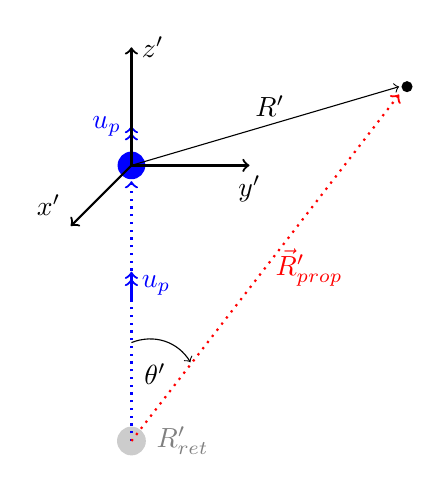
\begin{tikzpicture}[scale=5] 
\draw[blue, thick,->>] (-0,0.36,0) -- (-0,0.43,0) node[midway, right]{$\Vec{u}_p$};
\draw[blue, thick,->>] (0,0.7,0) -- (0,0.8,0) node[left]{$\Vec{u}_p$};
\fill (0.7,0.9,0) circle (0.4pt);
\fill[blue] (0,0.7,0) circle (1pt);
\draw[gray!40,fill=gray!40] (0,0,0) circle (1pt);
\node[gray] at (0.13,0,0) {$\Vec{R}'_{ret}$};
\draw[black, thick,->] (0,0.7,0) -- (0.3,0.7,0) node[anchor=north]{$y'$};
\draw[black, thick,->] (0,0.7,0) -- (0,1,0) node[anchor=west]{$z'$};
\draw[black, thick,->] (0,0.7,0) -- (0,0.7,0.4) node[anchor=south east] {$x'$};
\node at (0.06,0.17,0) {$\theta '$};
\draw[->] (0,0.25,0) to[bend left=40] (0.15,0.2,0);
\draw[thick,blue,dotted,->] (0,0,0) -- (0,0.66,0);
\draw[red, thick, dotted,->] (0,0,0) -- (0.68,0.88,0) node[midway, right] {$\vec{R}'_{prop}$};
\draw[black,->] (0,0.7,0) -- (0.68,0.9,0) node[midway,above] {\text{ $\Vec{R}'$}};
\end{tikzpicture}
\caption{The diagram shows a particle $p$ in blue, moving at a velocity $\Vec{u}_p$, currently positioned at the origin of an axis, it shows light from the source that is currently at a position $\Vec{R'}$, this light has propagated from the source when it was at position $\Vec{R}'_{ret}$ in grey, this light had propagated from this retarded position, along $\Vec{R}'_{prop}$, shown in red, to get to its current position, at an angle of $\theta '$ to the Z-axis.  }
\label{fig: Retarded field outward field}
\end{figure}

As visualised in figure (\ref{fig: Retarded field outward field}). If we have a light source particle $p$, that is moving at velocity $\vec{u_p}=(0,0,u_p)$ along the Z-axis and is currently positioned at the origin of an axis at time $t'=0$ (here we are choosing to show it as a primed coordinate, but we are just preemptively doing this because it will make it easier to introduce the Lorentz transformations later, at the moment we are staying in the same frame and not special relativity is being used). then if we have light that has been propagated from the source to the coordinate $\Vec{R}'= (x',y',z')$ at this time, this light would of had to been emitted from $P$ at a previous/retarded point in time $T'_{ret}$, at a retarded coordinate $\Vec{R'}_{ret}= \Vec{u}_p T'_{ret}=(0,0,u_p T'_{ret})$, such that the light has propagated along

\begin{equation}%%%%%%%%%%%%%%%
\label{displacement}
    \Vec{R'}_{prop} = -\Vec{c}'T'_{ret} = \Vec{R'} - \vec{R}'_{ret} =  \begin{pmatrix}
    x'\\ y' \\ z' - u_p T'_{ret}
    \end{pmatrix},
\end{equation}%%%%
to $\Vec{R'}$.


To find this retarded time, we will start with the magnitude of the propagation displacement from previous equation which is equal to the distance the light, propagating at the speed of light, $c$, travels in the corresponding propagation time $T'_{prop}=-T'_{ret}$. This gives

\begin{equation}%%%%%%%%%%%%%%%
        \begin{split}
        \left( c T_{prop}'\right)^2  = \left( -c T_{ret}'\right)^2 &= \|\Vec{R'}_{prop}\|^2 \\
        &= (x'^2 + y'^2 + z'^2) + u_p^2 T_{ret}'^2 - 2u_p z' T_{ret}',
%        (c^2 - v^2) T_{ret}'^2 &=  (x'^2 + y'^2 + z'^2) + 2v T_{ret}'z'
        \end{split}
\end{equation}%%%%

rearranging this, we get the quadratic

\begin{equation}%%%%%%%%%%%%%%%
        T_{ret}'^{2} + \left(2\gamma^2\frac{u_p}{c^2} z'\right)T_{ret}' - \frac{\gamma^2}{c^2}(x'^2+y'^2+z'^2) = 0,
\end{equation}%%%%

where $\gamma = (1 - u_p^2/c^2)^{-1/2}$, we may be preemptively using the constant $\gamma$ here but we have still not used any special relativity. Now taking the solution for the past time (negative solution) using the quadratic formula, and making use of the identity

\begin{equation}%%%%%%%%%%%%%%%
\label{eq: gamma identity}
    \gamma^2 = 1+\gamma^2\frac{u_p^2}{c^2},
\end{equation}%%%%

we get the result

\begin{equation}%%%%%%%%%%%%%%%
\label{Retarded Time}
    \begin{split}
    T_{ret}' &= -\gamma^2\frac{u_p}{c^2}z' - \sqrt{\left(-\gamma^2\frac{u_p}{c^2} z'\right)^2+\frac{\gamma^2}{c^2}(x'^2+y'^2+z'^2)} \\
    &= -\gamma^2\frac{u_p}{c^2}z' - \frac{\gamma}{c}\sqrt{x'^2+y'^2+\left(1+\gamma^2\frac{u_p^2}{c^2}\right) z'^2}\\
    &= - \gamma^2\frac{u_p}{c^2}z' - \frac{\gamma}{c}\sqrt{x'^2+y'^2+\gamma^2 z'^2} \\
    &= - \gamma^2\frac{u_p}{c^2}z' - \frac{\gamma}{c}\|\vec{R}\|.
    \end{split}
\end{equation}%%%%

Now in the final step, we finally introduced special relativity, with the lorentz transform we requiring $t'= 0$ for all coordinates, meaning that the primed and proper axis overlap at this time, and taking the primed frame as moving at velocity $v=-u_p$ along the z-axis relative to the proper frame of particle, and hence used the Lorentz transform of the spatial coordinates; $\vec{R}=(x,y,z)=(x',y',\gamma z')$, to get $\|\vec{R}\|$. With this we can rewrite the Z-component of equation (\eqref{displacement}) as
\begin{equation}%%%%%%%%%%%%%%%
    z' - u_p T_{ret}' \Rightarrow \gamma\left(z + \frac{u_p\cdot \|\vec{R}\|}{c}\right),
\end{equation}%%%%
giving the propagation displacement vector to be
\begin{equation}%%%%%%%%%%%%%%% 
\label{retarded displacement}
    \Vec{R}'_{prop}= \begin{pmatrix}
    x\\ y \\ \gamma \left(z + \dfrac{u_p \cdot \|\vec{R}\|}{c}\right)
    \end{pmatrix} = \|\vec{R}\|\begin{pmatrix}
    \frac{x}{\|\vec{R}\|}\\ \frac{y}{\|\vec{R}\|} \\ \gamma \left( \frac{z}{\|\vec{R}\|} + \dfrac{u_p}{c} \right)\\
    \end{pmatrix}.
\end{equation}%%%%
Since the light propagates along this in the primed frame, the unit vector of the primed propagation velocity at any general primed coordinate can be worked out to be (show working out in appendix) 
\begin{equation}%%%%%%%%%%%%%%% 
\label{eq: unit retarded velocity}
    \hat{\mathbf{\vec{U}'}} = \hat{\mathbf{\vec{R}'}}_{prop} = \dfrac{1}{\text{\AA}} \begin{pmatrix}
    \frac{x}{\|\vec{R}\|}\\ \frac{y}{\|\vec{R}\|} \\ \gamma \left( \frac{z}{\|\vec{R}\|} + \dfrac{u_p}{c} \right)
    \end{pmatrix},
\end{equation}%%%%
where the factor
\begin{equation}%%%%%%%%%%%%%%%
    \text{\AA} = \gamma\left( 1 + \frac{u_p}{c}\frac{z}{\|\vec{R}\|} \right). 
\end{equation}%%%%
Now taking the magnitude of the light propagation displacement from equation (\eqref{retarded displacement}) and using equation (\eqref{eq: gamma identity}), we have
\begin{equation}%%%%%%%%%%%%%%%
\label{eq: field displacement transform}
    \begin{split}
    \|\Vec{R}'_{prop}\|^2 &= x^2+y^2 + \gamma^2\left( z^2 +\frac{u_p^2}{c^2}\|\vec{R}\|^2 + 2 \frac{u_p}{c}z \|\vec{R}\| \right) \\
    &= \gamma^2 \|\vec{R}\|^2 + \frac{u_p^2}{c^2}\gamma^2z^2 + 2 \frac{u_p}{c}\gamma^2 z \|\vec{R}\| \\
    &= \gamma^2\left( \|\vec{R}\| + \frac{u_p}{c}z \right)^2\\
    &= \gamma^2\left( 1 + \frac{u_p}{c}\frac{z}{\|\vec{R}\|} \right)^2 \|\vec{R}\|^2 \\
    &= \text{\AA}^2 \|\vec{R}\|^2
    .
    \end{split}
\end{equation}%%%%
Since the luminal speed of the propagation will be same in both frames we have
\begin{equation}%%%%%%%%%%%%%%%
\label{eq: retarded field displacement transform}
\begin{split}
   c = \frac{\|\Vec{R}\|}{T_{prop}} &= \frac{\|\Vec{R}'_{prop}\|}{T_{prop}'}\\
    &=  \frac{\text{\AA}\|\Vec{R}\|}{T_{prop}'} \\
    T_{prop}' &= \text{\AA} T_{prop},
\end{split}
\end{equation}%%%%

where $T_{prop}$ is the proper (particles rest frame) time the light takes to propagate to $\vec{R}$ from the particle. 


... is this correct to say?... Time and length are stretched in the primed frame along $\vec{R}'_{ret}$ relative to the proper frame along $\vec{R}$ by a factor $\text{\AA}$, leading to the relative radial density of the light in the primed frame to that of the proper frame, which we will refer to as the radial light strength weighting, given as
\begin{equation}%%%%%%%%%%%%%%%
\label{eq: radial weighting}
    W_\rho = \frac{1}{\text{\AA}}.
\end{equation}%%%% 

%███████████████████████████████████████████████████████████████████
%███████████████████████████████████████████████████████████████████
\section{Acceleration}
*** gotta check which theta  this is
\subsection{General Equation}

\begin{equation}%%%%%%%%%%%%%%%
    \vec{a'} = \dfrac{1}{\gamma^2}\left[ \vec{a_0}+\left(\dfrac{1}{\gamma}-1\right)\left(\vec{a_0}\cdot\hat{\vec{v}}\right)\hat{\vec{v}}\right]
\end{equation}%%%%

\subsection{Co-moving Charges}

\begin{equation}%%%%%%%%%%%%%%%
    \vec{v} =  \begin{pmatrix}
    o\\ 
    v
    \end{pmatrix} =
    \begin{pmatrix}
    o\\ 
    -u_p
    \end{pmatrix}
\end{equation}%%%%

\begin{equation}%%%%%%%%%%%%%%%
    \vec{a_0} = \dfrac{k}{R^2} \begin{pmatrix}
    \sin\theta\\ 
    \cos{\theta}
    \end{pmatrix}
\end{equation}%%%%
Substituting into general equation

\begin{equation}%%%%%%%%%%%%%%%
    \vec{a'} = \dfrac{1}{\gamma^3}\dfrac{k}{R^2}\left[ \begin{pmatrix}
    \gamma\sin\theta\\ 
     \cos{\theta}
    \end{pmatrix} \right]
\end{equation}%%%%
\begin{equation}%%%%%%%%%%%%%%%
    \begin{split}
   \|\vec{a}'\| &=  \dfrac{1}{\gamma^2}\dfrac{k}{R^2}\sqrt{
    \sin^2\theta +
     \gamma^{-2}\cos^2{\theta}} \\
     &=  \dfrac{1}{\gamma^2}\dfrac{k}{R^2} \sqrt{
    \sin^2\theta +
     (1-\beta^2)\cos^2{\theta}} \\
     &=  \dfrac{1}{\gamma^2}\dfrac{k}{R^2} \sqrt{
    1 -\beta^2\cos^2{\theta}}
    \end{split}
\end{equation}%%%%
using trigonometry and retarded distance transform from above

\begin{equation}%%%%%%%%%%%%%%%
    \begin{split}
   \|\vec{a}'\| &=  \dfrac{1}{\gamma^2}\dfrac{k}{R^2} \sqrt{1 -\beta^2\cos^2{\theta}}\\
   &= \dfrac{1}{\gamma^2}\dfrac{k}{R^2} \sqrt{1 -\beta^2 \dfrac{(\cos\theta' + \beta)^2}{(1+\beta\cos\theta')^2}}\\
   &= \dfrac{1}{\gamma^2}\dfrac{k}{R^2} \sqrt{  \dfrac{(1+\beta\cos\theta')^2 - \beta^2(\cos\theta' + \beta)^2}{(1+\beta\cos\theta')^2}}\\
   &= \dfrac{1}{\gamma^2}\dfrac{k}{R^2} \sqrt{  \dfrac{(1+2\beta\cos\theta') - \beta^2(\beta^2 + 2 \beta\cos\theta')}{(1+\beta\cos\theta')^2}}\\
   &= \dfrac{1}{\gamma^2}\dfrac{k}{R^2} \sqrt{  \dfrac{(1-\beta^2)2\beta\cos\theta' + (1 - \beta^4)}{(1+\beta\cos\theta')^2}}
    \end{split}
\end{equation}%%%%


\begin{equation}%%%%%%%%%%%%%%%
\begin{split}
\vec{a'} &= \dfrac{1}{\gamma^3( 1+\beta\cos\theta')} \dfrac{k}{R^2} \begin{pmatrix}
    \sin\theta' \\ 
     \cos\theta' + \beta
    \end{pmatrix}\\
    &= \dfrac{1}{\gamma^3( 1+\beta\cos\theta')} \dfrac{k\left(\gamma\left(1+\beta\cos\theta^{'}\right)\right)^{-2}}{{R'_{ret}}^2} \begin{pmatrix}
    \sin\theta' \\ 
     \cos\theta' + \beta
    \end{pmatrix}\\
    &= \dfrac{1}{\gamma^5( 1+\beta\cos\theta')^3} \dfrac{k}{{R'_{ret}}^2} \begin{pmatrix}
    \sin\theta' \\ 
     \cos\theta' + \beta
    \end{pmatrix}
\end{split}
\end{equation}%%%%

\begin{equation}%%%%%%%%%%%%%%%
    \begin{split}
   \|\vec{a'}\| &=  \dfrac{1}{\gamma^3( 1+\beta\cos\theta')} \dfrac{k}{R^2} 
    \sqrt{\sin^2\theta' + (\cos\theta' + \beta)^2} \\   &= \dfrac{1}{\gamma^3( 1+\beta\cos\theta')} \dfrac{k}{R^2} 
    \sqrt{ 1 + \beta^2 +  2\cos\theta'\beta}
    \end{split}
\end{equation}%%%%

%███████████████████████████████████████████████████████████████████
%███████████████████████████████████████████████████████████████████
\section{Derivation from Spherical Light Pulse} \label{spherical light pulse derivation}%%%%%%%%%%%%%

*** what about reverse of the spherical wave derivation, so that the spherical pulse of light is emitted towards the origin to reach at time $t=0=t'$ (then it would be as if was emitted into the past if we continue the the propagation back through the origin)

***
If you have a point $r$ in an inertial frame then a spherical wave pulse would take $t= |r|/c$ to get there, we will call the light being at coordinate $r$ an event, now to find the corresponding event in the primed frame

*** free to choose the origin of the primed frame, so choosing it to be coinciding at the point light is emitted

***
maybe derive from spherical pulse on lorry, having it return and have its walls be general coordinates, with time dilation


*** derivation in words first:
- 2 inertial frames coinciding at $t=t'=0$ with primed frame moving relativity in z-direction
- Describe spherical wave pulse in proper frame and primed frame $|\vec{R}|=ct$ and $|\vec{R'}|=ct'$
- 




...





An observer is at the origin of an inertial frame of reference/coordinate system $<S>$. An object moving at a constant velocity $v$ relative to $<S>$ can be described to be stationary in an inertial frame of reference $<S'>$ moving the at the same velocity $v$ shown in Fig. \ref{ltrans}. 

\begin{figure}[ht]
\begin{tikzpicture}[scale=3]%,tdplot_main_coords]
\coordinate (O) at (0,0,0);
%
\draw (0,2,0) node{$t=0$};
\draw (-0.8,2,0) node{ {\large $<S>$}};
\draw[black, thick,->] (-0.2,0,0) -- (0.8,0,0) node[anchor=north east]{$x$};
\draw[black, thick,->] (0,-0.2,0) -- (0,0.8,0) node[anchor=north west]{$z$};
\draw[black, thick,->] (0,0,0.3) -- (0,0,-1) node[anchor=south]{$y$}; 
\draw[gray,dashed, thick,->] (-0.2,0,0) -- (0.4,0,0) node[anchor=north east]{$x'$};
\draw[gray,dashed, thick,->] (0,-0.2,0) -- (0,0.4,0) node[anchor=south west]{$z'$};
\draw[gray,dashed, thick,->] (0,0,0.3) -- (0,0,-0.5) node[anchor=south]{$y'$}; 
\draw[gray, thick, ->>] (-0.15,0,0) -- (-0.15,0.22,0) node[anchor=east]{$v$}; 
\fill[red] (0.65,0.2,0) circle (0.6pt);
\draw[gray, thick, ->>] (0.65,0.2,0) -- (0.65,0.42,0) node[anchor=west]{$v$}; 
%
\draw (1.7,2,0) node{$t>0$};
\draw[black, thick,->] (1.5,0,0) -- (2.5,0,0) node[anchor=north east]{$x$};
\draw[black, thick,->] (1.7,-0.2,0) -- (1.7,0.8,0) node[anchor=north west]{$z$};
\draw[black, thick,->] (1.7,0,0.3) -- (1.7,0,-1) node[anchor=south]{$y$}; 
%
\draw[gray, dashed, thick,->] (1.5,1.2,0) -- (2.2,1.2,0) node[anchor=north east]{$x'$};
\draw[gray, dashed, thick,->] (1.7,1,0) -- (1.7,1.7,0) node[anchor= west]{$z'$};
\draw[gray, dashed, thick,->] (1.7,1.2,0.3) -- (1.7,1.2,-0.8) node[anchor=south]{$y'$}; 
\draw[gray, thick, ->>] (1.55,1.2,0) -- (1.55,1.42,0) node[anchor=east]{$v$};
\fill[red] (2.35,1.4,0) circle (0.6pt);
\draw[gray, thick, ->>] (2.35,1.4,0) -- (2.35,1.62,0) node[anchor=west]{$v$}; 
%
\end{tikzpicture}
\caption{Proper frame of reference in standard configuration.}
\label{ltrans}
\end{figure}

\begin{figure}[H]
\begin{tikzpicture}[scale=3]%,tdplot_main_coords]
\coordinate (O) at (0,0,0);
%
\draw (0,1,0) node{$t'=0$};
\draw (-0.8,1,0) node{ {\large $<S'>$}};
\draw[black, thick,->] (-0.2,0,0) -- (0.8,0,0) node[anchor=north east]{$x'$};
\draw[black, thick,->] (0,-0.2,0) -- (0,0.8,0) node[anchor=north west]{$z'$};
\draw[black, thick,->] (0,0,0.3) -- (0,0,-1) node[anchor=south]{$y'$}; 
\draw[gray,dashed, thick,->] (-0.2,0,0) -- (0.4,0,0) node[anchor=north east]{$x$};
\draw[gray,dashed, thick,->] (0,-0.2,0) -- (0,0.4,0) node[anchor=south west]{$z$};
\draw[gray,dashed, thick,->] (0,0,0.3) -- (0,0,-0.5) node[anchor=south]{$y$}; 
\draw[gray, thick, ->>] (-0.15,0,0) -- (-0.15,-0.22,0) node[anchor=east]{$-v$}; 
\fill[red] (0.65,0.4,0) circle (0.6pt);
\fill[red] (2.35,0.4,0) circle (0.6pt);
%
\draw (1.7,1,0) node{$t'>0$};
\draw[black, thick,->] (1.5,0,0) -- (2.5,0,0) node[anchor=north east]{$x'$};
\draw[black, thick,->] (1.7,-0.2,0) -- (1.7,0.8,0) node[anchor=north west]{$z'$};
\draw[black, thick,->] (1.7,0,0.3) -- (1.7,0,-1) node[anchor=south]{$y'$}; 
%
\draw[gray, dashed, thick,->] (1.5,-0.9,0) -- (2.2,-0.9,0) node[anchor=north east]{$x$};
\draw[gray, dashed, thick,->] (1.7,-1.1,0) -- (1.7,-0.4,0) node[anchor= west]{$z$};
\draw[gray, dashed, thick,->] (1.7,-0.9,0.3) -- (1.7,-0.9,-0.8) node[anchor=south]{$y$}; 
\draw[gray, thick, ->>] (1.55,-0.9,0) -- (1.55,-1.12,0) node[anchor=east]{$-v$}; 
%
\end{tikzpicture}
\caption{Primed frame of reference in standard configuration.}
\end{figure}

\begin{itemize}
\setlength\itemsep{0em}

\item We start with setting the inertial frames up so that the origins of the Cartesian coordinates coincide at $t=0=t'$

\item It is chosen that the frame of reference $<S'>$ moves in the z-direction (this is chosen as it is easier to move to spherical polar coordinates later and since there is symmetry in the coordinates perpendicular to the movement, and having right-left symmetry is more visually simple)

\item *** if there is a spherical light pulse at the time the coordinate axis overlap at $t=t'=0$ such that the distance that the light has propagated at a time $t$ is $ct$ and $ct'$ respectfully so that the equation describing the spherical pulse in each frame is $ct = \sqrt{ x^2 + y^2 + z^2 }$ and $ct' = \sqrt{ x'^2 + y'^2 + z'^2 }$

\item We define the $s$ and $s'$ as:

\vspace{-1cm}
\begin{equation}%%%%%%%%%%%%%%%
\begin{split}
 s^2 &= -c^2t^2 + x^2 + y^2 + z^2 \\  s'^2 &= -c^2t'^{2} + x'^2 + y'^2 + z'^2 
\end{split}
\label{s}
\end{equation}%%%%

*** Diagram of wave fronts with both axis in same diagram one moving relative to other showing  (maybe having 2 diagrams one with each frame of reference at rest) ***

\item At an expanding wave front moving at the speed of light $c$, in the two frames we have $s= s'=0$

\item We are therefore looking for a transformation s.t. $s=0 \Leftrightarrow s'=0$ 

\item for a linear transform it is implied $s'^2= k s^2$ (where k is a constant) ** why does it have to be linear? (to allow for smooth inverse transformation)

\item By symmetry $ s^2=k^2 s'^2=k^2 s^2$ which leads to $ k^2= 1 \Rightarrow k=1$ ( $k=-1$ is disallowed because as $v\rightarrow 0$ we must recover $s=s'$ )

\item So $s'^2=s^2$, and by symmetry $x'=x$, $y'=y$ (this is taken from the cannon and ball thought experiment from chapter...)

\item This leads to:
\vspace{0cm}
\begin{equation}%%%%%%%%%%%%%%%
\label{seqs}
-c^2t^2+ z^2 = -c^2t'^2 +z'^2
\end{equation}%%%%

\item The requirement $z'=0$ when $z=vt$, the form of a linear equation that gives this for all values of $t$ is
\vspace{0cm}
\begin{equation}%%%%%%%%%%%%%%%
\label{xbar}
z' = \gamma (z-vt) 
\end{equation}%%%%
\item where $\gamma$ is yet to be determined, we have chosen the linear equation and not one that depends on factors greater than first order, i.e. squared or greater terms of $(z-vt)$, this is because the linear... (to allow for smooth inverse transformation)

\item By symmetry if we wanted to instead transform from $<S'>$ to $<S>$, it is the same transform but with the frame change in the opposite direction, so $x,y,z,t$ can just be replaced by $x',y',z',t'$ when the sign in front of $v$ is also changed *** maybe diagram to show this

\item Substituting $z'$ into the inverse of eq. \eqref{xbar} leads to

\begin{equation}%%%%%%%%%%%%%%%
\label{ttrans}
    t'=\gamma \bigg[t-\frac{z}{v}\bigg(1-\frac{1}{\gamma^2}\bigg)\bigg]
\end{equation}%%%%

\item Subbing the previous two equations into eq. \eqref{seqs} gives

\begin{equation}%%%%%%%%%%%%%%%
    -c^2t^2+ z^2 = -c^2\gamma^2\bigg[ t -\frac{z}{v}\bigg(1-\frac{1}{\gamma^2}\bigg)\bigg]^2 + \gamma^2(z-vt)^2
\end{equation}%%%%

\item This holds true for all $z$ and $t$ 
\item Equating terms ( this is a mathematical technique, were it is known that for an equation like this to be true for all values of $t$ it is required that all terms in front $t^2$ on each side of the equation must be equal) in front of $t^2$ leads to

\begin{equation}%%%%%%%%%%%%%%%
\mhl{
    \gamma= \frac{1}{\sqrt{1-\beta^2}}
    }
\end{equation}%%%%

\item Subbing this into previous equations now completes the Lorentz Transformation:


%\vspace{-1cm}
\begin{equation}%%%%%%%%%%%%%%%
\label{lorentz transformation 2}
\mhl{
    \begin{aligned}
      &  x'=x \\ & y'=y \\ &z' = \gamma (z-vt)  \\ 
       \text{From eq. \eqref{ttrans} \ \ \ } & t'=\gamma \bigg(t-\frac{vz}{c^2}\bigg)
    \end{aligned}
    }
\end{equation}%%%%
*** explain the time transform in terms of the gamma function being the slowing down part and the $\frac{vz}{c^2}$ being the "anti-simultaneity" part
%\vspace{-0.9cm}
\item Galilean coordinates obtained by letting $v\rightarrow 0$
\end{itemize}
we can write this in vector form, multiplying $t'$ by $c$ to give unit of length, this is known as the positional 4 vector and is given as
\begin{equation}%%%%%%%%%%%%%%% 
\label{spacial transform}
    \bf{R}'= \begin{pmatrix}
    ct' \\ x'\\ y' \\ z'
    \end{pmatrix} = \begin{pmatrix}
    \gamma\left( ct - \dfrac{vz}{c} \right) \\x\\ y \\ \gamma \left( z - vt \right)\\
    \end{pmatrix}.
\end{equation}%%%%
an event is given by its spacial coordinates and the time at which it happens.


%███████████████████████████████████████████████████████████████████
\section{Length Contraction}
%███████████████████████████████████████████████████████████████████
\section{Time Dilation}

Taking two times $t_1$ and $t_2$ of a clock at rest at position $z$ in one inertial frame will have transformed times in another reference frame of $t'_1 = \gamma(t_1 - \frac{v}{c^2}z_1)$ $t'_2 = \gamma(t_2 - \frac{v}{c^2}z_2)$ so that the difference in time is

\begin{equation}%%%%%%%%%%%%%%%
\begin{split}
   \Delta t' &=  t'_2 - t'_1 \\ &= \gamma(t_2 - \frac{v}{c^2}z) - \gamma(t_1 - \frac{v}{c^2}z) \\ &= \gamma (t_2 - t_1 ) \\ &= \gamma \Delta t
\end{split}
\end{equation}%%%%
when we take the change of time at the same location in a rest frame, we always have that $\Delta t' > \Delta t$ i.e the change in time in the rest frame of an observer corresponds to a greater change in time in another moving frame of reference.

%███████████████████████████████████████████████████████████████████
%███████████████████████████████████████████████████████████████████
\section{Generalised velocity vector transform}
%███████████████████████████████████████████████████████████████████
\subsection{god knows what this is: Doppler Effect}

%██████████
\begin{figure}[ht]
\begin{subfigure}{.49\textwidth}
  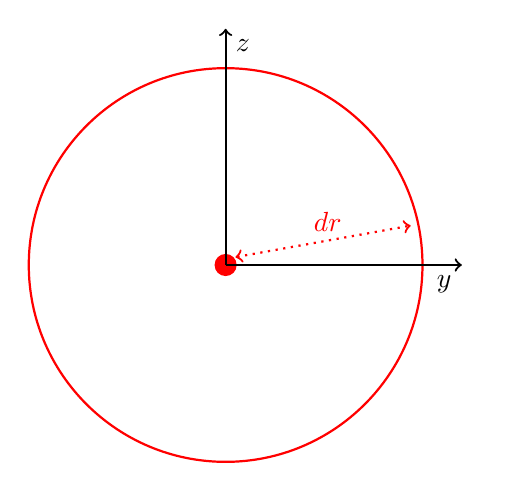
\begin{tikzpicture}[scale=5] 
\draw[white] (0,0.6,0) -- (0,-0.5,0);
\draw[white] (0.7,0) -- (-0.5,0);
\fill[red] (0,0,0) circle (0.8pt);
\draw[red,thick] (0 ,0) circle (0.5);
\draw[black, thick,->] (0,0,0) -- (0.6,0,0) node[anchor=north east]{$y$};
\draw[black, thick,->] (0,0,0) -- (0,0.6,0) node[anchor=north west]{$z$};
%\draw[->] (0,0.25/2,0) to[bend left=45] (0.21/2,0.04,0);
%\node at (0.08,0.17,0) {$\theta $};
\draw[red,thick, dotted,<->] (0.025,0.02,0) -- (0.47,0.1,0) node[midway,above] {\text{ $dr$}};
\end{tikzpicture}
\caption{Spherical pulse in rest frame}
%  \label{fig:sub1}
\end{subfigure}
\begin{subfigure}{.49\textwidth}
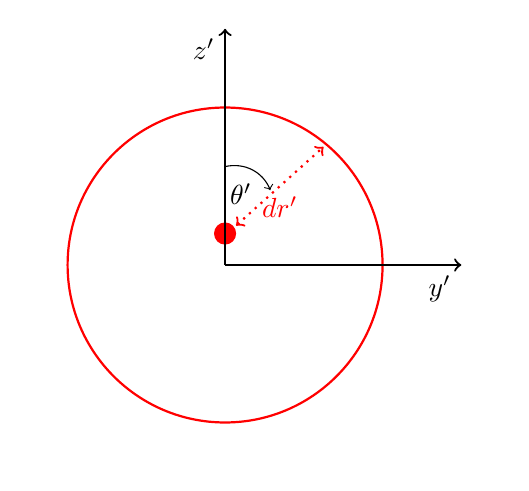
\begin{tikzpicture}[scale=5]
\draw[white] (0,0.6,0) -- (0,-0.5,0);
\draw[white] (0.7,0) -- (-0.5,0);
\fill[red] (0,0.08,0) circle (0.8pt);
\draw[red,thick] (0 ,0) circle (0.4);
\draw[thick,->] (0,0,0) -- (0.6,0,0) node[anchor=north east]{$y'$};
\draw[thick,->] (0,0,0) -- (0,0.6,0) node[anchor=north east]{$z'$};
\draw[red,thick, dotted,<->] (0.028,0.1,0) -- (0.25,0.3,0) node[midway, below] {$dr'$};
\draw[->] (0,0.25,0) to[bend left=40] (0.23/2,0.19,0);
\node at (0.04,0.18,0) {$\theta' $};
\end{tikzpicture}
\caption{Spherical pulse in Primed frame}
%  \label{fig:sub2}
\end{subfigure}
\caption{ since I have everything in opposite directions, need to change equations *** also this is full blown relativity not just retarded field }
\label{fig: Doppler effect appendix}
\end{figure}
%██████████
**** this is for receiving particle that is at rest, i.e. $u_p=0$ ****

Figure \ref{fig: Doppler effect appendix}, shows a particle emitting a spherical wave of light, in the proper frame it begins emitting at time $t=0$ and after an infinitesimal amount of time the front of the wave has spread out spherically, such that the front is at a distance $dr$ from the origin at all positions,while the wave continues to be emitted from the origin. In the primed frame the wavefront is emitted at $t'=0$ and reaches a point that is $\gamma dr$ from the origin at all points, with the gamma due to $dr=cdt$ and the the time $dt=\gamma dt'$, but we also now have to take into account that the source particle that is still emitting this wave has moved along the z'-axis to a point $u_p dt'= \gamma u_p dt$ and each part of the wave being emitted from the source is taken as being emitted at an angle $\theta'$, such that any point on the wavefront that is at and angle of $\theta'$ from the particle, will have the distance $dr'$ between it and the source, and the wave that is currently being emitted from the source particle will go to that position on the wavefront (offal description).

We can get the Doppler effect by taking the ratio of the distances the way will have to travel to get to the current point the wavefront is at, which in the rest frame is $dr=cdt$ and in the primed frame is $|d\vec{dr}'| = u_p/c \gamma dr$
%███████████████████████████████████████████████████████████████████
%███████████████████████████████████████████████████████████████████
\chapter{Todo for these notes}
* \AA \ \ is not the same \AA \ \ in velocity and acceleration transform as it is in time transform (( it is the same as its the retarded cosine angel which is same as cosine of angle for primed frame as its at the retarded position

(try to make it as readable as possible for people with poor English, or for the translation)

an introduction sentence... ((relativity cause its the theory of motion for objects relative to other objects, and special because its specifically for the special case where gravity's effects negligible and are not required to be included in calculations and objects are moving at constant velocities)) ((as gravity curves spacetime giving curved coordinates))

decide whether to include minkowski diagram as it is an abstract view rather than representational view

%███████████████████████████████████████████████████████████████████
%███████████████████████████████████████████████████████████████████
\section{A note on different notations}
*primed notation
* my notation for frames

3 postulates/ starting points.